\chapter{Feldquantisierung\label{chapter:feldquantisierung}}
\lhead{Feldquantisierung}
\begin{refsection}
\chapterauthor{Hannes Diethelm}

\printbibliography[heading=subbibliography]
\end{refsection}

\section{Einleitung}

Ziel dieses Kapitels ist, auf Basis der Maxwell-Gleichungen, der Fourier-Theorie und einer Quantisierung analog des harmonischen Oszillators (Kapitel \ref{chapter:harmonischeroszillator}) die Feldquantisierung f"ur elektromagnetische Wellen her zu leiten.

Auf Grund der Quantisierung werden somit aus elektromagnetischen Wellen Energiequanten, genannt Photonen, die mit Elektronen wechselwirken k"onnen. Die Form der Wechselwirkung l"asst unter anderem R"uckschl"usse zu, die praktisch in Lasern Verwendung finden.

Die Ausf"uhrungen in diesem Kapitel basieren gr"osstenteils auf: \cite{fq:aqm}

\section{Maxwell-Gleichungen und elektromagnetische Wellen}

Hilfreich dazu ist auch die Beschreibung von Magnetfeldern in Kapitel \ref{chapter:magnetfeld}. In diesem Kapitel wird der Gradient durch $\nabla$ ersetzt \cite{fq:nabla}.

Die in der Elektrotechnik wohl bekannten Maxwell-Gleichungen in SI Einheiten lauten:
\begin{align}
\nabla\cdot E &= \frac{\rho}{\varepsilon_0} \label{fq:maxwell_1},\\
\nabla\times B &= \mu_0 j  + \mu_0 \varepsilon_0\frac{\partial E}{\partial t} \label{fq:maxwell_2},\\
\nabla\cdot B &=0 \label{fq:maxwell_3},\\
\nabla\times E &= -\frac{\partial B }{\partial t} \label{fq:maxwell_4}.
\end{align}
Zudem gilt
\begin{equation*}
\mu_0\varepsilon_0=\frac{1}{c^2}.
\end{equation*}

In Kapitel \ref{section:vektorpotential} wurde gezeigt, dass $B$ als Rotation des Vektorpotentials $A$ geschrieben werden kann:
\begin{equation}
B = \nabla\times A,
\end{equation}
wodurch (\ref{fq:maxwell_3}) erf"ullt wird, da $\nabla \cdot ( \nabla\times V ) = 0$ f"ur jedes Vektorfeld V gilt. Also ist
\begin{equation*}
\nabla \cdot B = \nabla \cdot ( \nabla\times A ) = 0.
\end{equation*}

Wir definieren $E$ als
\begin{equation}
E = -\dfrac{\partial A}{\partial t} - \nabla \varphi.
\end{equation}
wobei $\varphi$ ist das skalare Potential des Feldes ist. Durch Einsetzen von $E$ in (\ref{fq:maxwell_4}) wird ersichtlich, dass die Gleichung damit erf"ullt ist:
\begin{equation*}
\nabla\times (-\dfrac{\partial A}{\partial t} - \nabla \varphi) + \frac{\partial \nabla\times A }{\partial t} = 
- \frac{\partial \nabla\times A }{\partial t} - \underbrace{\nabla\times \nabla \varphi}_{=0\text{ f"ur jedes Potential } \varphi} + \frac{\partial \nabla\times A }{\partial t} = 0.\\
\end{equation*}
(\ref{fq:maxwell_3}) und (\ref{fq:maxwell_4}) wurden bereits erf"ullt. Durch Einsetzen von $E$ und $B$ wird aus (\ref{fq:maxwell_1}) und (\ref{fq:maxwell_2}):
\begin{align} 
 \label{fq:a_coupled_a}
 \nabla^2 \varphi + \dfrac{\partial \nabla A}{\partial t} &= -\rho, \\
 \label{fq:a_coupled_b}
 \nabla^2 A - \frac{1}{c^2} \frac{\partial^2 A }{\partial t^2} - \nabla \left( \nabla \cdot A + \frac{1}{c^2} \frac{\partial \varphi }{\partial t} \right) &= - \frac{1}{c} j.
\end{align}
Die vier Maxwell-Gleichungen k"onnen also auch als zwei Gleichungen in $A$ und $\varphi$ dargestellt werden.
Mittels der Lorenz-Eichung (Siehe Kapitel \ref{section:eichtransformation}) kann $\varphi$ so gew"ahlt werden, dass
\begin{equation} \label{fq:lorenz_eq}
\nabla \cdot A + \frac{1}{c^2} \frac{\partial \varphi }{\partial t} = 0.
\end{equation}
Dadurch werden die zwei gekoppelten Gleichungen (\ref{fq:a_coupled_a}) und (\ref{fq:a_coupled_b}) entkoppelt und es gilt
\begin{align*}
\nabla^2 \varphi - \frac{1}{c^2} \dfrac{\partial^2 \varphi}{\partial t^2} &= -\rho, \\
\nabla^2 A - \frac{1}{c^2} \frac{\partial^2 A }{\partial t^2} &= - \frac{1}{c} j.
\end{align*}

F"ur die Feldquantisierung wollen wir ein freies Feld im Vakuum betrachten. Hierf"ur gilt $j = 0$ sowie $\rho = 0$.
Die Gleichung f"ur $\varphi$ wird nicht ben"otigt und die Gleichung f"ur $A$ wird zu
\begin{equation} \label{fq:wave_dgl}
\nabla^2 A - \frac{1}{c^2} \frac{\partial^2 A }{\partial t^2} = 0.
\end{equation}

\section{Vom Wellenfeld zu unabh"angigen Oszillatoren}
L"osungen dieser Gleichung f"ur periodische Randbedingungen und $t=0$ in einem W"urfel mit Seitenl"ange $L = V^{1/3}$ sind durch die Fourier-Reihe gegeben \cite{fq:em_wave_eq}:
\begin{equation} \label{fq:wave_eq}
A(x,t) = \frac{1}{\sqrt{V}} \sum_k \sum_{\alpha=1,2} \left(c_{k,\alpha} \varepsilon^{(\alpha)} e^{i (k \cdot x - \omega_k t)} + \bar{c}_{k,\alpha} \varepsilon^{(\alpha)} e^{-i(k \cdot x - \omega_k t)}\right).
\end{equation}
$k$ ist der Ausbreitungsvektor der Welle und zeigt in die Ausbreitungsrichtung und $\varepsilon^{(\alpha)}$ ist die Polarisation. Dabei ist:
\begin{align*}
\omega_k=|k|c, \\
\lambda = \frac{2 \pi}{|k|}.
\end{align*}
Durch setzen von $c_{k,\alpha}(t) = c_{k,\alpha} e^{-i \omega_k t}$ sowie $u_{k,\alpha}(x) = \varepsilon^{(\alpha)} e^{ik \cdot x}$ kann die Gleichung auch in Zeit- und Ortsabh"angige Faktoren aufgeteilt werden:
\begin{equation*}
A(x,t) = \frac{1}{\sqrt{V}} \sum_k \sum_{\alpha=1,2} \left(c_{k,\alpha}(t)u_{k,\alpha}(x) + \bar{c}_{k,\alpha}(t) \bar{u}_{k,\alpha}(x) \right).
\end{equation*}

$A(x,t)$ wird durch die konjugiert komplexe Wahl der Koeffizienten f"ur alle $c_{k,\alpha}$ reell:
\begin{equation*}
(a + ib)(\cos k \cdot x + i \sin k \cdot x ) + (a - ib)(\cos k \cdot x - i \sin k \cdot x ) = 2 ( a \cos k \cdot x - b \sin k \cdot x ).
\end{equation*}
%=a \cos k \cdot x + ib \cos k \cdot x + ia \sin k \cdot x - b \sin k \cdot x + a \cos k \cdot x - ib \cos k \cdot x - ia \sin k \cdot x - b \sin k \cdot x

Es stellt sich nun die Frage, wie die Vektoren $k$ und $\varepsilon^{(\alpha)}$ gew"ahlt werden m"ussen. Damit die Orthogonalit"at der Fourier-Reihe gew"ahrleistet ist, m"ussen $(\varepsilon^{(1)}, \varepsilon^{(2)} \text{ und } \varepsilon^{(3)})$ orthogonal sein. Wir w"ahlen die L"ange $1$. Durch Linearkombinationen k"onnen somit beliebige Polarisationen gew"ahlt werden. Zudem setzen wir fest, dass $\varepsilon^{(3)}$ sowie $k$ parallel sind.

Die Berechnung von $B$ liefert
\begin{equation*}
B = \nabla \times A = \frac{1}{ \sqrt{V}} \sum_{\alpha=1,2}  \sum_k i \underbrace{k \times \varepsilon^{(\alpha)}}_{\neq 0} \left(c_{k,\alpha} e^{i (k \cdot x - \omega_k t)} - \bar{c}_{k,\alpha} e^{-i(k \cdot x - \omega_k t)} \right).
\end{equation*}

Hier darf der Term $k \times \varepsilon^{(\alpha)}$ nicht verschwinden, damit sich eine Welle bilden kann. $\varepsilon^{(3)}$ f"allt weg, da das Vektorprodukt von parallelen Vektoren null ist. Wir definieren somit, dass $(\varepsilon^{(1)}, \varepsilon^{(2)} , k/|k|)$ ein orthogonales Rechtssystem aus Einheitsvektoren bilden.

Da $\varepsilon^{(\alpha)}$ und $k$ orthogonal sind, gilt
\begin{equation*}
\nabla \cdot A = \frac{1}{\sqrt{V}} \sum_k \sum_{\alpha=1,2} i \underbrace{k \cdot \varepsilon^{(\alpha)}}_{=0} \left(c_{k,\alpha} e^{i (k \cdot x - \omega_k t)} - \bar{c}_{k,\alpha} e^{-i(k \cdot x - \omega_k t)}\right) = 0.
\end{equation*}
Aufgrund der Lorenz-Eichung (\ref{fq:lorenz_eq}) gilt dadurch
\begin{equation*}
\frac{\partial \varphi }{\partial t} = - c^2 \nabla \cdot A = 0.
\end{equation*}

Die Berechnung von $E$ liefert
\begin{equation*}
	E = - \frac{\partial A}{\partial t} = \frac{1}{\sqrt{V}} \sum_k \sum_{\alpha=1,2} i \omega_k \varepsilon^{(\alpha)} \left(c_{k,\alpha} e^{i (k \cdot x - \omega_k t)} - \bar{c}_{k,\alpha} e^{-i(k \cdot x - \omega_k t)} \right).
\end{equation*}
Hier wird sichtbar, dass das $A$-Feld den selben Polarisations- sowie Ausbreitungsvektor hat, die Phase aber $90^\circ$ verschoben ist.

Weiterhin gilt wegen der Orthogonalit"at der komplexen Exponentialfunktion auch:
\begin{align*}
\dfrac{1}{V} \int u_{k,\alpha} \cdot \bar{u}_{k',\alpha'} d^3 x &= \delta_{kk'}\delta{aa'}, \\
\dfrac{1}{V} \int u_{k,\alpha} \cdot u_{k',\alpha'} d^3 x &= 0, \\
\dfrac{1}{V} \int \bar{u}_{k,\alpha} \cdot \bar{u}_{k',\alpha'} d^3 x &= 0.
\end{align*}

Die Hamilton-Funktion einer elektromagnetischen Welle ist gegeben durch
\begin{equation*}
\begin{split}
H &= \frac{1}{2} \int \left(\frac{1}{\mu_0}|B|^2 + \varepsilon_0|E|^2\right) d^3 x \\
	&= \frac{1}{2} \int \left(c^2 \varepsilon_0 | \nabla\times A |^2 + \varepsilon_0 \left| \dfrac{\partial A}{\partial t} \right|^2 \right) d^3 x.
\end{split}
\end{equation*}
Es kann gezeigt werden, dass die L"osung dieses Integrals gegeben ist durch
\begin{equation*}
H = \sum_k \sum_{\alpha=1,2} 2 \varepsilon_0 \omega_k^2 \bar{c}_{k,\alpha}(t) c_{k,\alpha}(t).
\end{equation*}
Durch 
\begin{equation*}
Q_{k,\alpha} = \sqrt{\varepsilon_0} \left(c_{k,\alpha}(t) + \bar{c}_{k,\alpha}(t)\right) \quad \text{und} \quad P_{k,\alpha} = -i \omega_k \sqrt{\varepsilon_0} \left(c_{k,\alpha}(t) - \bar{c}_{k,\alpha}(t)\right)
\end{equation*}
wird die Hamilton-Funktion zu
\begin{equation} \label{fq:hamilton}
\begin{split}
H &= \sum_k \sum_{\alpha=1,2} 2 \omega_k^2 
	\underbrace{\left[ \frac{\omega_k Q_{k,\alpha} - i P_{k,\alpha}}{2 \omega_k} \right]}_{\sqrt{\varepsilon_0} \bar{c}_{k,\alpha}(t)}
	\underbrace{\left[ \frac{\omega_k Q_{k,\alpha} + i P_{k,\alpha}}{2 \omega_k} \right]}_{\sqrt{\varepsilon_0} c_{k,\alpha}(t)} \\
&= \sum_k \sum_{\alpha=1,2} \frac{1}{2} \left(P_{k,\alpha}^2 + \omega_k^2 Q_{k,\alpha}^2\right).
\end{split}
\end{equation}

Hier sieht man nun, dass es m"oglich ist, eine Welle durch unabh"angige Oszillatoren dar zu stellen.
$Q_{k,\alpha}$ und $P_{k,\alpha}$ k"onnen nun als Koordinaten und Impulse der einzelnen Oszillatoren aufgefasst werden:
\begin{equation*}
\dfrac{\partial H}{\partial Q_{k,\alpha}} = -\dot{P}_{k,\alpha}, \qquad \dfrac{\partial H}{\partial P_{k,\alpha}} = \dot{Q}_{k,\alpha}.
\end{equation*}

\section{Quantisierung des Wellenfeldes}

Die im vorigen Kapitel hergeleitete Darstellung des Wellenfeldes als einzelne unabh"angige Oszillatoren l"asst die Interpretation dieser wie in Kapitel \ref{chapter:harmonischeroszillator} beschrieben, zu. Dadurch ist eine analoge Quantisierung m"oglich, die es erlaubt, Wechselwirkungen zwischen dem Feld und Elektronen zu beschreiben.

Analog zum harmonischen Oszillator werden zuerst die Vertauschungsrelationen und die Auf- und Absteige-Operatoren hergeleitet und dann die Wirkung auf die Zustandsvektoren berechnet. Dies ist praktisch identisch zum harmonischen Oszillator, nur geht es hier um elektromagnetische Wellen.

\subsection{Vertauschungsrelationen sowie Auf- und Absteige-Operatoren}
Wie beim harmonischen Oszillator k"onnen $Q_{k,\alpha}$ und $P_{k,\alpha}$ nun als Operatoren aufgefasst werden. Die Vertauschungsrelationen werden dabei zu
\begin{align*}
[Q_{k,\alpha}, P_{k',\alpha'}] &= i \hbar \delta_{kk'}\delta_{aa'}, \\
[Q_{k,\alpha}, Q_{k',\alpha'}] &= 0, \\
[P_{k,\alpha}, P_{k',\alpha'}] &= 0.
\end{align*}

Wir definieren die Operatoren:
\begin{align*}
a_{k,\alpha} &= \frac{1}{\sqrt{2 \hbar \omega_k}} (\omega_k Q_{k,\alpha} + iP_{k,\alpha}), \\
a^+_{k,\alpha} &= \frac{1}{\sqrt{2 \hbar \omega_k}} (\omega_k Q_{k,\alpha} - iP_{k,\alpha}),\\
\begin{split}
N_{k,\alpha} &= a^+_{k,\alpha} a_{k,\alpha} = \frac{1}{2 \hbar \omega_k} \left(P_{k,\alpha}^2 + \omega_k^2 Q_{k,\alpha}^2 + i\omega_k [Q_{k,\alpha},P_{k,\alpha}] \right) \\
 &= \frac{1}{ \hbar \omega_k } H - \frac{1}{2} = {\cal H} - \frac{1}{2}.
\end{split}
\end{align*}
Ein Vergleich mit (\ref{fq:hamilton}) liefert
\begin{equation} \label{fq:opp_fourier}
 c_{k,\alpha} \rightarrow \sqrt{\frac{\hbar}{2 \varepsilon_0 \omega_k}} a_{k,\alpha}, \qquad 
 \bar{c}_{k,\alpha} \rightarrow \sqrt{\frac{\hbar}{2 \varepsilon_0 \omega_k}} \, a^+_{k,\alpha}.
\end{equation}
Somit entsprechen diese Operatoren den Fourier-Koeffizienten.

Die Kommutatoren f"ur diese Operatoren sind
\begin{align*}
\begin{split}
[a_{k,\alpha} , a^+_{k',\alpha'}] &= - \frac{i}{2 \hbar} [Q_{k,\alpha}, P_{k',\alpha'}] + \frac{i}{2 \hbar} [P_{k,\alpha}, Q_{k',\alpha'}] \\
	 &= \delta_{kk'}\delta_{aa'},
\end{split}\\
[a_{k,\alpha} , a_{k',\alpha'}] &= [a^+_{k,\alpha} , a^+_{k',\alpha'}] = 0, \\
\begin{split}
[a_{k,\alpha} , N_{k',\alpha'}] &= a_{k,\alpha} a^+_{k',\alpha'} a_{k',\alpha'} - a^+_{k',\alpha'} a_{k',\alpha'} a_{k,\alpha} \\
	&= [a_{k,\alpha} , a^+_{k',\alpha'}]a_{k',\alpha'} - a^+_{k',\alpha'}[a_{k',\alpha'} , a_{k,\alpha}]\\
	&= \delta_{kk'}\delta_{aa'} a_{k,\alpha},
\end{split} \\
[a^+_{k,\alpha} , N_{k',\alpha'}] &= -\delta_{kk'}\delta_{aa'} a^+_{k,\alpha}.
\end{align*}

\subsection{Wirkung auf Zustandsvektoren}

In diesem Unterkapitel werden Suffixes $k$ und $\alpha$ weggelassen, da wir nur die Wirkung der Operatoren auf einen einzelnen Oszillator betrachten. 

Diese Operatoren werden nun wie beim harmonischen Oszillator auf den Zustand angewendet. Wir suchen einen Eigenvektor $|n\rangle$ und Eigenwert $e_n$ zum Operator $N$ so dass
\begin{equation*}
N|n\rangle = e_n|n\rangle.
\end{equation*}
Auf Grund der Beziehungen der Operatoren gilt dadurch
\begin{align*}
Na^+|n\rangle &= (a^+N + a^+)|n\rangle = (e_n + 1)a^+|n\rangle, \\
Na|n\rangle &= (aN - a)|n\rangle = (e_n - 1)a|n\rangle.
\end{align*}

Die Auf- und Absteige Operatoren f"ugen also dem quantisierten Feld Energiequanten hinzu oder entfernen solche.

Wiederum m"ussen die neuen Eigenvektoren normalisiert werden. Daf"ur werden die Konstanten $c_+$ und $c_-$ eingef"uhrt:
\begin{align*}
a^+|n\rangle &= c_+|n+1\rangle, \\
a|n\rangle &= c_-|n-1\rangle.
\end{align*}
$c_\pm$ wird folgendermassen berechnet:
\begin{align*}
\begin{split}
	|c_+|^2 &= |c_+|^2 \langle n+1 \, | \, n+1 \rangle = ( a^+ \langle n |\,) \; a^+ \,| n \rangle \\
		&= \langle n |\, a \, a^+ \,|n \rangle = \langle n |\, N + [a,a^+] \,|n \rangle \\
		&= e_n+1,
\end{split}\\
	|c_-|^2 &= 	( a \langle n |\,) \; a \,| n \rangle = \langle n |\, a^+ a \,| n \rangle = e_n.
\end{align*}
Die Phase von $c_{\pm}$ ist nicht definiert. Sie kann auf null bei $t=0$ gesetzt werden. Bei $t=0$ gilt
\begin{align*}
a^+\,|n\rangle &= \sqrt{e_n+1}\,|n+1\rangle, \\
a\,|n\rangle &= \sqrt{e_n}\,|n-1\rangle.
\end{align*}

Da die Energie nicht negativ sein kann, gilt
\begin{equation*}
e_n = \langle n |\, N \,|n \rangle = \langle n |\, a^+a \,|n \rangle \geq 0.
\end{equation*}

Hier muss $n$ ein Integer sein, damit die absteigende Folge bei null stehen bleibt. Die absteigende Folge der Zust"ande ist
\begin{equation*}
a\,|n\rangle = \sqrt{e_n}\,|n-1\rangle  \;, \quad \hdots \; , \quad a\,|2\rangle = \sqrt{2}\,|1\rangle \; , \quad a\,|1\rangle = 0\,|0\rangle \;, \quad a\,|0\rangle = 0\,|0\rangle.
\end{equation*}

Hier ist der kleinst m"ogliche Eigenwert $e_n = 0$. Dem aufmerksamen Beobachter ist aufgefallen, dass der kleinste Eigenwert bei harmonischen Oszillator $e_n = \frac{1}{2}$ ist. Dies r"uhrt daher, dass wie hier f"ur $N$ Eigenwerte gesucht haben, im Kapitel \ref{chapter:harmonischeroszillator} aber f"ur ${\cal H}$. Die Korrektheit der Formeln gilt f"ur beide Operatoren. Der Grund liegt darin, dass der Nullpunkt der Energieskala nicht festgelegt ist und f"ur die Feldquantisierung keine Rolle spielt. Es gibt Anwendungen wie bei der Gravitation, wo der Nullpunkt nicht frei w"ahlbar ist. Wo dieser genau liegt ist stand der aktuellen Forschung.

\subsection{Photonen}

Die mit den Auf- und Absteige-Operatoren hinzugef"ugten und entfernten Energiequanten entsprechen den von Einstein in einer Publikation zum photoelektrischen Effekt vorausgesagten Energiequanten und werden Photonen genannt. Da das Verhalten von Elektronen und Photonen quantenmechanisch betrachtet sehr "ahnlich ist, k"onnen Photonen auch als Teilchen betrachtet werden.

Die hergeleitete Algebra kann nun auf ein Feld von Photonen, in dem die Anzahl Photonen mit bestimmter Polarisation ($\alpha$) und Impuls (Wellenl"ange $|k|$ sowie Ausbreitungsrichtung $k$) vergr"ossert oder verkleinert wird, angewendet werden.

Der Eigenvektor von $N_{k,\alpha}$ ist der Zustandsvektor f"ur einen Zustand mit einer bestimmten Anzahl Photonen im Zustand $(k,\alpha)$. $n_{k,\alpha}$ ist dabei die Besetzungszahl f"ur den Zustand $(k,\alpha)$. Der Vakuum-Zustand ist $|0\rangle$. Mit dem Aufsteige-Operator k"onnen nun Photonen hinzugef"ugt werden:

\begin{align*}
a^+_{k,\alpha}|0\rangle & \quad \text{f"ur ein Photon,}\\
\left(1/\sqrt{2}\right)a^+_{k_1,\alpha_1}a^+_{k_2,\alpha_2}|0\rangle & \quad \text{f"ur zwei Photonen}
\end{align*}
oder allgemein:
\begin{equation*}
|n_{k_1,\alpha_1}, n_{k_2,\alpha_2}, \, \hdots \, , n_{k_l,\alpha_l}\rangle =
 \prod_{k_i,\alpha_i}\underbrace{\frac{1}{\sqrt{n_{k_i,\alpha_i}}}}_{\text{Normierung}} \underbrace{\left(a^+_{k_i,\alpha_i}\right)^{n_{k_i,\alpha_i}}}_{\text{Aufsteigeoperator}} |0\rangle.
\end{equation*}

Die Fourier-Koeffizienten im Strahlungsfeld werden mittels den Korrespondenzen (\ref{fq:opp_fourier}) durch Operatoren ersetzt um das quantisierte Feld zu erhalten:
\begin{equation*}
A(x,t) = \frac{1}{\sqrt{V}} \sum_k \sum_{\alpha=1,2} \sqrt{\frac{\hbar}{2 \varepsilon_0 \omega_k}} \left[a_{k,\alpha} \varepsilon^{(\alpha)} e^{i (k \cdot x - \omega_k t)} + a^+_{k,\alpha} \varepsilon^{(\alpha)} e^{-i (k \cdot x - \omega_k t)}\right].
\end{equation*}

Durch die Definition zeitabh"angiger Operatoren
\begin{align*}
a_{k,\alpha}(t) &= a_{k,\alpha} e^{-i \omega_k t}, &
u_{k,\alpha}(x) &= \varepsilon^{(\alpha)} e^{ik \cdot x}, \\
a^+_{k,\alpha}(t) &= a^+_{k,\alpha} e^{i \omega_k t}, &
\bar{u}_{k,\alpha}(x) &= \varepsilon^{(\alpha)} e^{-ik \cdot x}.
\end{align*}
kann die Gleichung wiederum in Zeit- und Ortsabh"angige Faktoren aufgeteilt werden:
\begin{equation*}
A(x,t) = \frac{1}{\sqrt{V}} \sum_k \sum_{\alpha=1,2} \sqrt{\frac{\hbar}{2 \varepsilon_0 \omega_k}}\left[a_{k,\alpha}(t) u_{k,\alpha}(x) + a^+_{k,\alpha}(t) \bar{u}_{k,\alpha}(x) \right].
\end{equation*}

Auch wenn diese Gleichung mit (\ref{fq:wave_eq}) verwandt ist, ist die Bedeutung sehr verschieden. Erstere ist eine klassische Funktion in $x$ und $t$. Diese Gleichung ist nun ein Operator aus Linearkombinationen von Auf- und Absteigeoperatoren f"ur jeden Punkt im Raum. Ein solcher Operator heisst {\em Feldoperator} oder {\em quantisiertes Feld}.

\subsubsection{Feldenergie}
Der Hamiltonoperator ist nun
\begin{equation*}
H = \frac{1}{2} \int \left(\frac{1}{\mu_0} B \cdot B + \varepsilon_0 E \cdot E \right) d^3 x.
\end{equation*}

Dieses Integral kann wiederum ausgewertet werden, nur muss dieses mal die Reihenfolge von $a_{k,\alpha}$ und $a^+_{k,\alpha}$ eingehalten werden:
\begin{equation*}
\begin{split}
H &= \frac{1}{2} \sum_k \sum_{\alpha=1,2} \hbar \omega_k \left(a^+_{k,\alpha} a_{k,\alpha} + a_{k,\alpha} a^+_{k,\alpha}\right) \\
&= \sum_k \sum_{\alpha=1,2} \hbar \omega_k \left(N_{k,\alpha} + \frac{1}{2} \right).
\end{split}
\end{equation*}

Die absolute Energieskala ist hier wiederum frei w"ahlbar. Durch die Wahl von $H|0\rangle = 0$ folgt
\begin{equation*}
H = \sum_k \sum_{\alpha=1,2} \hbar \omega_k N_{k,\alpha}.
\end{equation*}

Der Hamiltonoperator angewendet auf viele Photonen ergibt nun als Eigenwert die Summe der Energie der Photonen mit den Zust"anden $(k_i,\alpha_i)$:
\begin{equation*}
H |n_{k_1,\alpha_1}, n_{k_2,\alpha_2}, \, \hdots\rangle = \sum_i \hbar \omega_k n_{k_i,\alpha_i} |n_{k_1,\alpha_1}, n_{k_2,\alpha_2}, \, \hdots\rangle.
\end{equation*}

\section{Wechselwirkung zwischen Photonen und Elektronen}

In diesem Kapitel wird das Ziel erreicht, die Wechselwirkung zwischen Photonen und Elektronen zu beschreiben. Durch diese Beschreibung k"onnen die Einstein-Koeffizienten einfach hergeleitet werden.

Zwischen Photonen und den Neutronen und Protonen eines Atomkerns gibt es zwar auch eine Wechselwirkung. Da die Kernzust"ande sehr viel h"ohere Energien beinhalten, w"aren f"ur eine Zustands"anderung Photonen weit "uber der Gammastrahlung n"otig. Zudem befinden sich viele Elektronen um den Kern, die den Kern praktisch abschirmen und somit viel eher mit den Photonen wechselwirken als der Kern.

Der Spin von Photonen und Elektronen wird vernachl"assigt, da dieser Einfluss zwar vorhanden, aber sehr klein ist.

\subsection{Hamiltonoperator}

Der allgemeine Hamiltonoperator ist
\begin{equation*}
H = \frac{1}{2m}p^2 + V(x).
\end{equation*}

Um den Hamiltonoperator eines Elektrons im Feld zu erhalten, wird $p$ gem"ass Kapitel \ref{section:hamilton-funktion-im-magnetfeld} durch $p - eA$ ersetzt. $A$ ist nun das quantisierte Feld. Der Hamiltonoperator wird somit zu
\begin{equation*}
\begin{split}
H &= \frac{1}{2m}(p - eA)^2 + V(x)\\
 &= \underbrace{\frac{1}{2m}p^2 + V(x)}_{H_0} + \underbrace{\frac{1}{2m}\left[- e p \cdot A(x, t) - e A(x, t) \cdot p + e^2 A(x, t) \cdot A(x, t) \right]}_{H_{\text{int}}}.
\end{split}
\end{equation*}

$p$ ist ein Operator mit Ableitung nach dem Ort. Da $\nabla \cdot A = 0$ gilt, vertauschen $p \cdot A(x, t)$.  Dadurch wird der Wechselwirkungs-Hamilton zu
\begin{equation*}
H_{\text{int}} = -\frac{e}{m} A(x, t) \cdot p + \frac{e^2}{2m}A(x, t) \cdot A(x, t).
\end{equation*}

Es interessieren uns sp"ater nur die Interaktionen mit einen Anfangszustand $X$ und Endzustand $Y$, also der Form $\langle Y| \, H \, |X \rangle$. Der Anfangszustand und der Endzustand sind orthogonal.

$H_0$ ist der Hamilton-Opperator f"ur das Elektron ohne das elektromagnetische Feld. Es gilt
\begin{equation*}
\langle Y| \, H \, |X \rangle = \langle Y| \, H_0 + H_{\text{int}} \, |X \rangle = \langle Y| \, H_0 \, |X \rangle + \langle Y| \, H_{\text{int}} \, |X \rangle.
\end{equation*}

Da $X$ und $Y$ verschiedene Eigenzust"ande des Elektrons, und somit von $H_0$, sind gilt $\langle Y| \, H_0 \, |X \rangle=0$. Wir nur m"ussen also nur $\langle Y| \, H_{\text{int}} \, |X \rangle$ betrachten.

\subsection{Wechselwirkung zwischen Photonen und Elektronen}

Wir wollen nun die Wechselwirkung zwischen Elektronen und Photonen herleiten. Dieser Hamiltonoperator wirkt nun nicht nur auf dem Zustand des Elektrons sondern auch auf den Zust"anden der Photonen und beschreibt die Wechselwirkung von Photonen und Elektronen.

Nehmen wir an, ein Elektron absorbiert ein Photon vom Zustand $(k,\alpha)$ und wechselt dabei vom Zustand $X$ in den Zustand $Y$. Der Einfachheit halber ber"ucksichtigen wir nur Photonen im Zustand $(k,\alpha)$. Der quadratische Term $A \cdot A$ spielt hier keine Rolle, da dieser Term nur Zustands"anderungen von $0$ oder $\pm 2$ Photonen erzeugt. Die Beschreibung der Zustands"anderung des Absorptionsprozesses ist
\begin{equation} \label{fq:absorbtion}
\begin{split}
\langle Y; n_{k,\alpha} - 1 |\, H_{\text{int}} \,| X; n_{k,\alpha} \rangle &=
 -\frac{e}{m} \left\langle Y; n_{k,\alpha} - 1 \biggl| 
 \, \frac{1}{\sqrt{V}} \sqrt{\frac{\hbar}{2 \varepsilon_0 \omega_k}}a_{k,\alpha} \varepsilon^{(\alpha)} e^{i(k \cdot x-\omega_k t)} \cdot p \,
\biggl| X; n_{k,\alpha} \right\rangle\\
&= -\frac{e}{m} \sqrt{\frac{n_{k,\alpha} \hbar}{2 \varepsilon_0 \omega_k V}} \left\langle Y \left|
\, e^{ik \cdot x} \varepsilon^{(\alpha)} \cdot p \,
\right| X \right\rangle e^{-i\omega_k t}.
\end{split}
\end{equation}

Der Emissionsprozess wird beschrieben durch
\begin{equation} \label{fq:emission}
\begin{split}
\langle Y; n_{k,\alpha} + 1 |\, H_{\text{int}} \,| X; n_{k,\alpha} \rangle &= 
-\frac{e}{m} \left\langle Y; n_{k,\alpha} + 1 \biggl| 
\, \frac{1}{\sqrt{V}} \sqrt{\frac{\hbar}{2 \varepsilon_0 \omega_k}}a^+_{k,\alpha} \varepsilon^{(\alpha)} e^{-i(k \cdot x-\omega_k t)} \cdot p \,
\biggl| X; n_{k,\alpha} \right\rangle\\
&= -\frac{e}{m} \sqrt{\frac{ (n_{k,\alpha}+1) \hbar}{2 \varepsilon_0 \omega_k V}} \left\langle Y \left| 
\, e^{-ik \cdot x} \varepsilon^{(\alpha)} \cdot p \,
\right| X \right\rangle e^{i\omega_k t}.
\end{split}
\end{equation}

Die Wahrscheinlichkeit eines "Uberganges ist gegeben durch $| \langle Y| \, H_{\text{int}} \, |X \rangle |^2$.
Somit ist die Wahrscheinlichkeit einer Absorption proportional zu $n_{k,\alpha}$ und einer Emission zu $n_{k,\alpha}+1$.

\subsection{Folgerungen}
\subsubsection{Emission und Absorption}
Beim Betrachten von (\ref{fq:emission}) f"allt auf, dass die Wahrscheinlichkeit f"ur die Emission bei nicht vorhandener elektromagnetischer Strahlung ($n_{k,\alpha} = 0$) gr"osser als null ist, da $n_{k,\alpha}+1 > 0$. Dieses Ph"anomen wird spontane Emission genannt.

Bei st"arkerer Strahlung ist die Wahrscheinlichkeit der Emission ungef"ahr proportional zur Anzahl Photonen und wird stimulierte Emission genannt. Da die emittierten Photonen exakt den selben Zustand haben wie anregenden, kann dieses Ph"anomen dazu verwendet werden, einen Laser zu bauen, bei dem alle ausgesendeten Photonen den selben Zustand haben. Dies wird in Kapitel \ref{chapter:laser} beschrieben.

Die Absorption ist proportional zur Anzahl Photonen. Wenn das Feld gen"ugend stark ist ($n_{k,\alpha} \gg 1$) ist die Absorptions- sowie Emissionswahrscheinlichkeit praktisch gleich, da $n_{k,\alpha}+1 \approx n_{k,\alpha}$. 

\subsubsection{Einsteinkoeffizienten}
Es befinden sich $n_1$ Atome im Grundzustand $1$ sowie $n_2$ Atome im angeregten Zustand $2$. Das Feld hat die spektrale Strahldichte $\rho(\lambda)$. Einstein definierte die Koeffizienten $B_{12}$, $B_{21}$ sowie $A_{21}$ so dass
\begin{itemize}
	\item die Rate der Absorption durch $\dfrac{dn_2}{dt} = B_{12} n_1 \rho(\lambda)$,
	\item die Rate der stimulierten Emission durch $\dfrac{dn_1}{dt} = B_{21} n_2 \rho(\lambda)$ und
	\item die Rate der spontanen Emission f"ur $\rho(\lambda)=0$ durch $\dfrac{dn_1}{dt} = A_{21} n_2$
\end{itemize}
gegeben ist. Diese Koeffizienten werden Einsteinkoeffizienten \cite{fq:einstein_koeff} genannt und zur Berechnung der spontanen und stimulierten Emission sowie der Absorption verwendet.

Diese Vorg"ange sind auch in Abbildung~\ref{fq_img:abs} und \ref{fq_img:em} dargestellt.

Mit den Ausf"uhrungen in diesem Kapitel ist auf einfache Art gezeigt, dass $B_{12} = B_{21}$ f"ur $\rho(\lambda) \gg 0$ gilt sowie dass eine spontane Emission ($A_{21} > 0$) existiert.

\begin{figure}
	\centering
	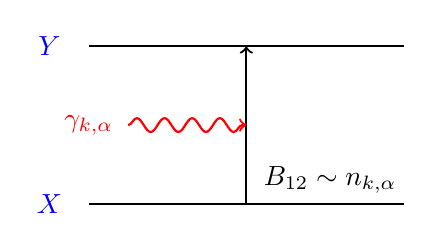
\begin{tikzpicture}
	\node[color=blue] at (0, 0) {$X$};	
	\node[color=blue] at (0, 2) {$Y$};
	\node[color=red] at (0.5, 1) {$\gamma_{k,\alpha}$};
	\node[color=black,anchor=west] at (2.6, 0.3) {$B_{12} \sim n_{k,\alpha}$};
	
	\draw[color=black,thick] (0.5, 0) -- +( 4, 0);
	\draw[color=black,thick] (0.5, 2) -- +( 4, 0);
	\draw[->,color=black,thick] (2.5, 0) -- +( 0, 2);	
	\draw[->,decorate, decoration={snake},color=red,thick] (1, 1) -- +( 1.5, 0);
	\end{tikzpicture}
	\caption{Absorption eines Photons
		\label{fq_img:abs}}
\end{figure}

\begin{figure}
	\centering
	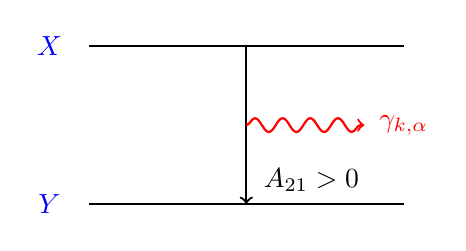
\begin{tikzpicture}
	\node[color=blue] at (0, 0) {$Y$};	
	\node[color=blue] at (0, 2) {$X$};
	\node[color=red] at (4.5, 1) {$\gamma_{k,\alpha}$};
	\node[color=black,anchor=west] at (2.6, 0.3) {$A_{21} > 0$};
	
	\draw[color=black,thick] (0.5, 0) -- +( 4, 0);
	\draw[color=black,thick] (0.5, 2) -- +( 4, 0);
	\draw[->,color=black,thick] (2.5, 2) -- +( 0, -2);	
	\draw[->,decorate, decoration={snake},color=red,thick] (2.5, 1) -- +( 1.5, 0);
	\end{tikzpicture}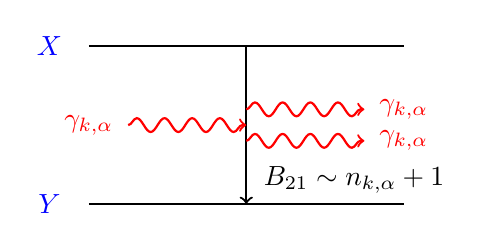
\begin{tikzpicture}
	\node[color=blue] at (0, 0) {$Y$};	
	\node[color=blue] at (0, 2) {$X$};
	\node[color=red] at (0.5, 1) {$\gamma_{k,\alpha}$};
	\node[color=red] at (4.5, 0.8) {$\gamma_{k,\alpha}$};
	\node[color=red] at (4.5, 1.2) {$\gamma_{k,\alpha}$};
	\node[color=black,anchor=west] at (2.6, 0.3) {$B_{21} \sim n_{k,\alpha} + 1$};
	
	\draw[color=black,thick] (0.5, 0) -- +( 4, 0);
	\draw[color=black,thick] (0.5, 2) -- +( 4, 0);
	\draw[->,color=black,thick] (2.5, 2) -- +( 0, -2);
	\draw[->,decorate, decoration={snake},color=red,thick] (1, 1) -- +( 1.5, 0);
	\draw[->,decorate, decoration={snake},color=red,thick] (2.5, 0.8) -- +( 1.5, 0);
	\draw[->,decorate, decoration={snake},color=red,thick] (2.5, 1.2) -- +( 1.5, 0);
	\end{tikzpicture}
	\caption{Spontane und stimulierte Emission eines Photons
		\label{fq_img:em}}
\end{figure}
